%
% main.tex - a typical phil presentation
%
% Copyright (c) 2015, Phil Maker
% GPLv2 
% 
%    

\documentclass{beamer}
%\documentclass[a4paper,handout]{beamer}
%\usepackage{pgfpages}
%\pgfpagesuselayout{4 on 1}[a4paper,border shrink=5mm]

\mode<presentation>{\usetheme{Pjm}}
\usepackage{graphics}
\usepackage{fancyvrb}
\newenvironment{code}
{\Verbatim[fontfamily=courier,%
numbers=right,stepnumber=5,%
firstnumber=\the\inputlineno]}%
{\endVerbatim}
\usepackage[english]{babel}
%\usepackage[latin1]{inputenc}
\usepackage{hyperref}
\definecolor{links}{HTML}{2A1B81}
\hypersetup{
  pdftitle = {Southern Exposure: an overview of PV/Diesel in
  Malaysia and Australia},
  pdfsubject = {PV Diesel}
  pdfkeywords = {Energy, Renewables, Powerwater, Phil Maker},
  pdfauthor = {\textcopyright\ Phil Maker, ...},
  pdfcreator = {\LaTeX\ with package \flqq hyperref \frqq},
  colorlinks,linkcolor=,urlcolor=links
}
\usepackage{xcolor}
\definecolor{JungleGreen}{cmyk}{0.99,0,0.52,0}
\definecolor{BlueGreen}{cmyk}{0.85,0,0.33,0}
\definecolor{RawSienna}{cmyk}{0,0.72,1,0.45}
\def\dill#1{\textcolor{RawSienna}{\textbf{Dill Alert: #1}}}

\title{Southern Exposure: an overview of PV/Diesel in Korea, Malaysia and
  Australia} 
\author{Phil Maker\\
  \href{mailto:philip.maker@gmail.com}{\texttt{<philip.maker@gmail.com>}}
}
\institute{Alaskan Center for Energy and Power}
\date{March 2015}
\logo{
\includegraphics[height=0.7cm]{logo.jpg}}
\begin{document}

\begin{frame}
  \maketitle
  \vspace{-0.6cm}
  \begin{abstract}
    \small A summary of some efforts in the PV/Diesel/Battery
    area including solar forecasting.This is a meta talk which is
    intended to mostly lead to other material (nothing original is
    presented by the humble author).
  \end{abstract}
\end{frame}

\section{Overview}
\begin{frame}\frametitle{Overview}
Overview of PV/Diesel/Battery work in:
 
  \begin{enumerate}
  \item Korea
  \item Australia
  \item Malaysia 
  \item Sky Cameras and Solar Forecasting
  \end{enumerate}
\pause
Finally: the talk is sourced from a number 
of kind people and is open source.
\pause
\vfill
\begin{quote}
``Remember that every view,
\pause\\
is based on where you are looking from'' -- Uncle Phil
\end{quote}
\end{frame}

\section{Australia}
\begin{frame}\frametitle{ARENA}
  ARENA \href{www.arena.gov.au}{www.arena.gov.au} has approximately
  \$2.5 billion in funding in order to:
  \begin{enumerate}
  \item Fund renewable energy projects
  \item Support research and development activities
  \item Support activities to capture and share knowledge
  \end{enumerate}
\pause
Projects larger than 26M\$:
\begin{itemize}
\item AGL Solar Project 166M\$
\item Australian Solar Thermal Research Initiative 35M\$
\item Australia-US Institute for Advanced Photovoltaics 33M\$
\item Cooper Basin Enhanced Geothermal Systems Heat/Power 59M\$
\item Kogan Creek Solar Boost project 34M\$
\item Moree Solar Farm 101M\$
\item NT SETuP Program 27M\$ (or 55M\$ total project)
\end{itemize}
\end{frame}

\begin{frame}\frametitle{Northern Territory: SETuP} 
  \begin{itemize}
  \item $>$30 sites medium penetration with 9MW PV and no storage.
    \pause
    Intended to reach 60\% peak penetration/contribution with a fuel
    saving of around 15\%.
  \item Single 1MW PV/Diesel/Battery system running diesel off (or 200\%
    penetration in Alaskan) with an intended fuel saving of around 50\%.
  \item Aiming to change both the organisation and the technology.
  \end{itemize}
  \pause
  \begin{itemize}
  \item Medium Penetration Rollout
  \item Sky Camera Forecasting (now casting)
  \item Demand Management using Saturn South kit (see Tim Warren).
  \end{itemize}
  \pause
  Main point to note is that: 35 x anything is a lot, 35 x 2w for
  commissioning means a few years work.

  Contact: \href{mailto:andrew.gray@powerwater.com.au}{Andrew Gray}
\end{frame}

% Malaysia
\section{Malaysia and Indonesia}
\begin{frame}\frametitle{Malaysia and Indonesia}

\begin{itemize}
\item Sabah and Sarawak - lots of isolated native communities similar
  to AK/AU-north.\pause
\item Indonesia - similar challenges across 
  a vast number of islands. \pause
\item Government hybrid power systems running diesel with battery
  storage.
\pause 
\end{itemize}
\pause
Its worth looking at:
\begin{itemize}
\item Optimal Power Solutions
  (\href{www.optimal-power-solutions.com}{www.optimal-power-solutions.com})
\item LEONICS (\href{www.leonics.com}{www.leonics.com}) 
\pause
\item Others...
\end{itemize}
\end{frame}

\begin{frame}\frametitle{Minigrid}
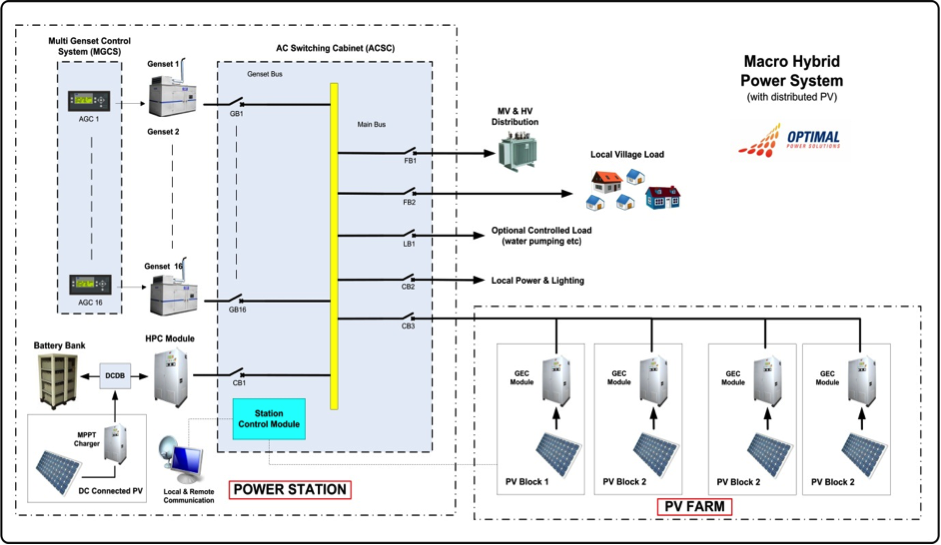
\includegraphics[width=\hsize]{optimal_power_macro_hybrid_mini_grid_line_diagram_ops.png}
\end{frame}

% Korea
\section{Korea}
\begin{frame}\frametitle{KEPCO Gasado Island}
  \begin{itemize}
  \item Population of 286, in southern South Korea.
  \item Load: 61..95..173 kW.
  \item Aim: 99\% Renewable Energy, mixed PV, battery, diesel storage.
  \item Running since last year. 
  \end{itemize}
\pause
  \begin{enumerate}
  \item KEPCO - Korean Electric Power Company (largest utility in S. Korea).
  \item Contact/Author: Wookyu Chae
    \href{wkchae@kepco.co.kr}{wkchae@kepco.co.kr} who kindly provided
    the next few slides.
  \item The complete presentation is available as well and is quite interesting.
  \end{enumerate}
\end{frame}

\begin{frame}\frametitle{Single Line Diagram}
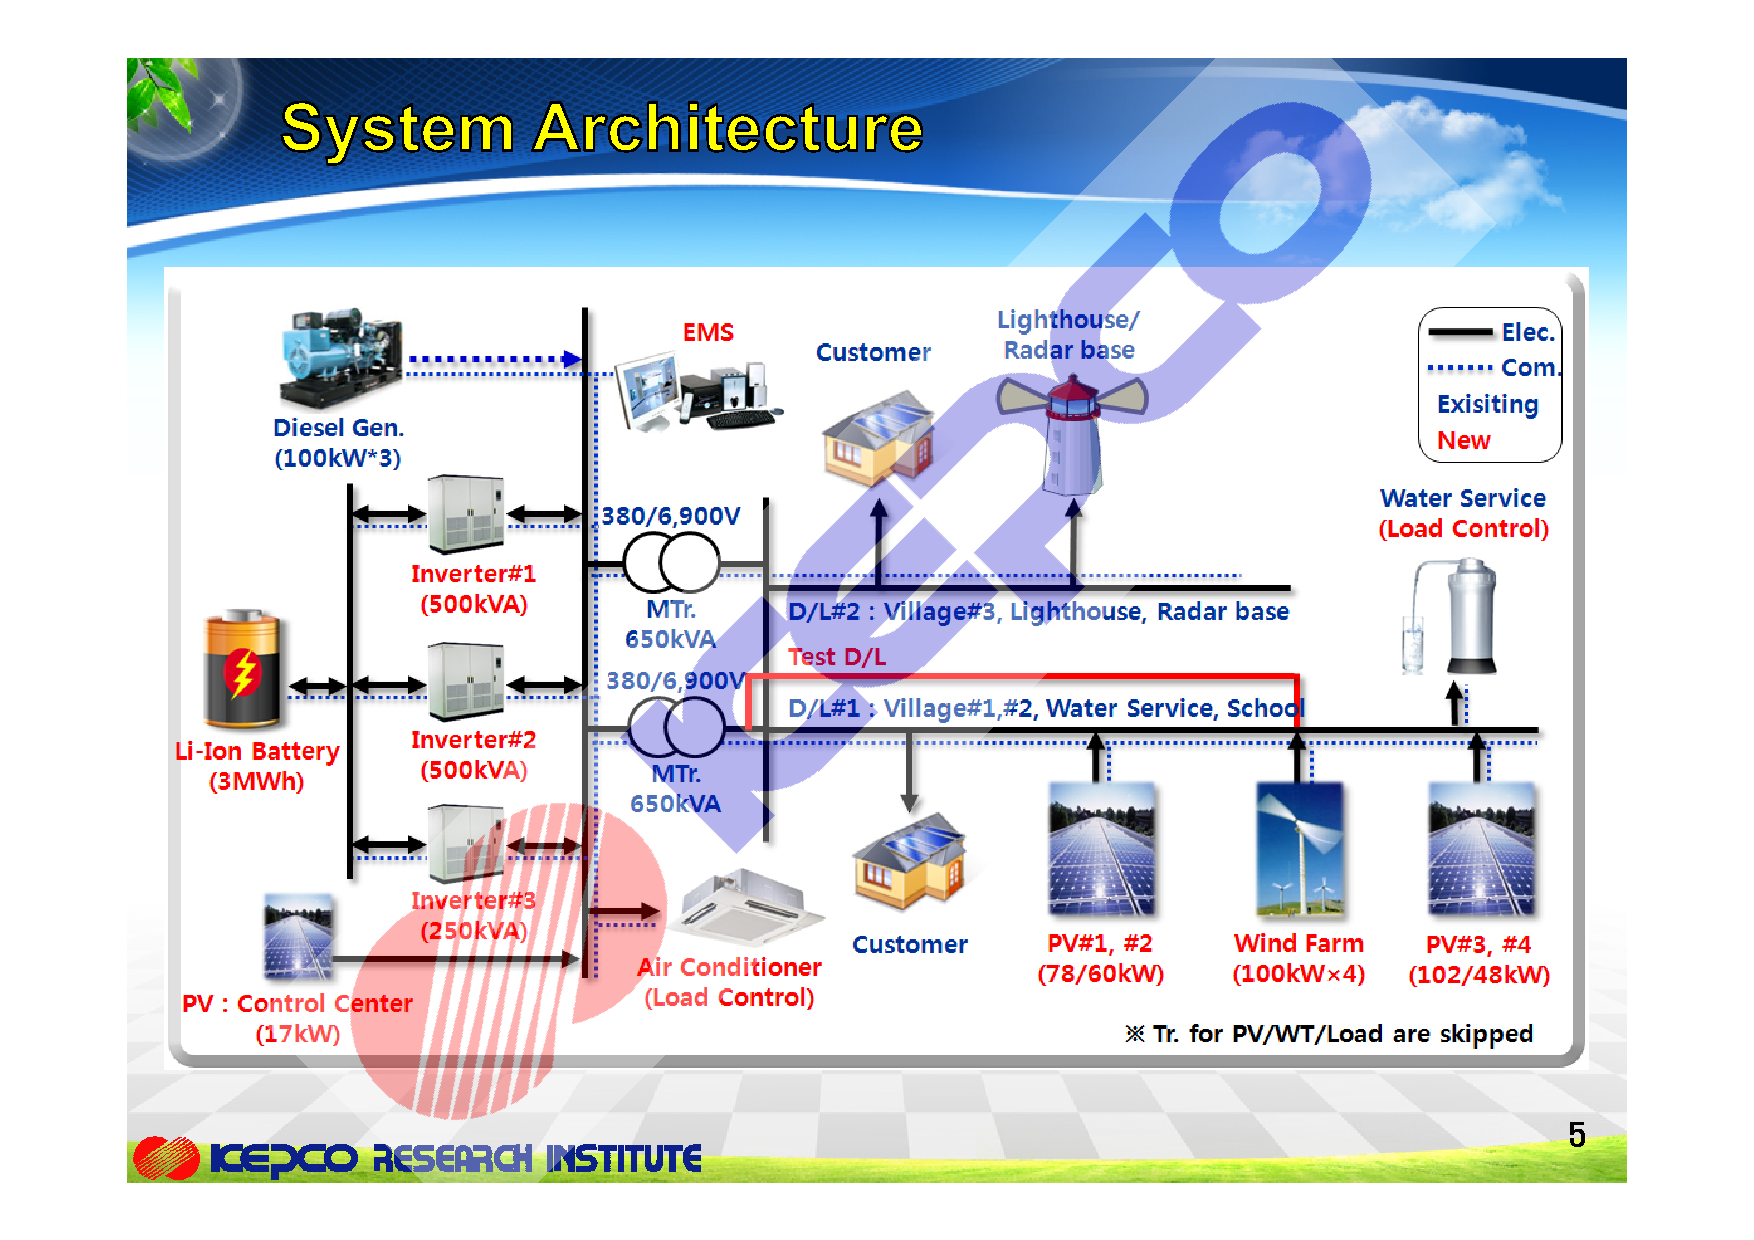
\includegraphics[width=\hsize]{KEPCO-SLD.pdf}
\end{frame}

\begin{frame}\frametitle{Equipment}
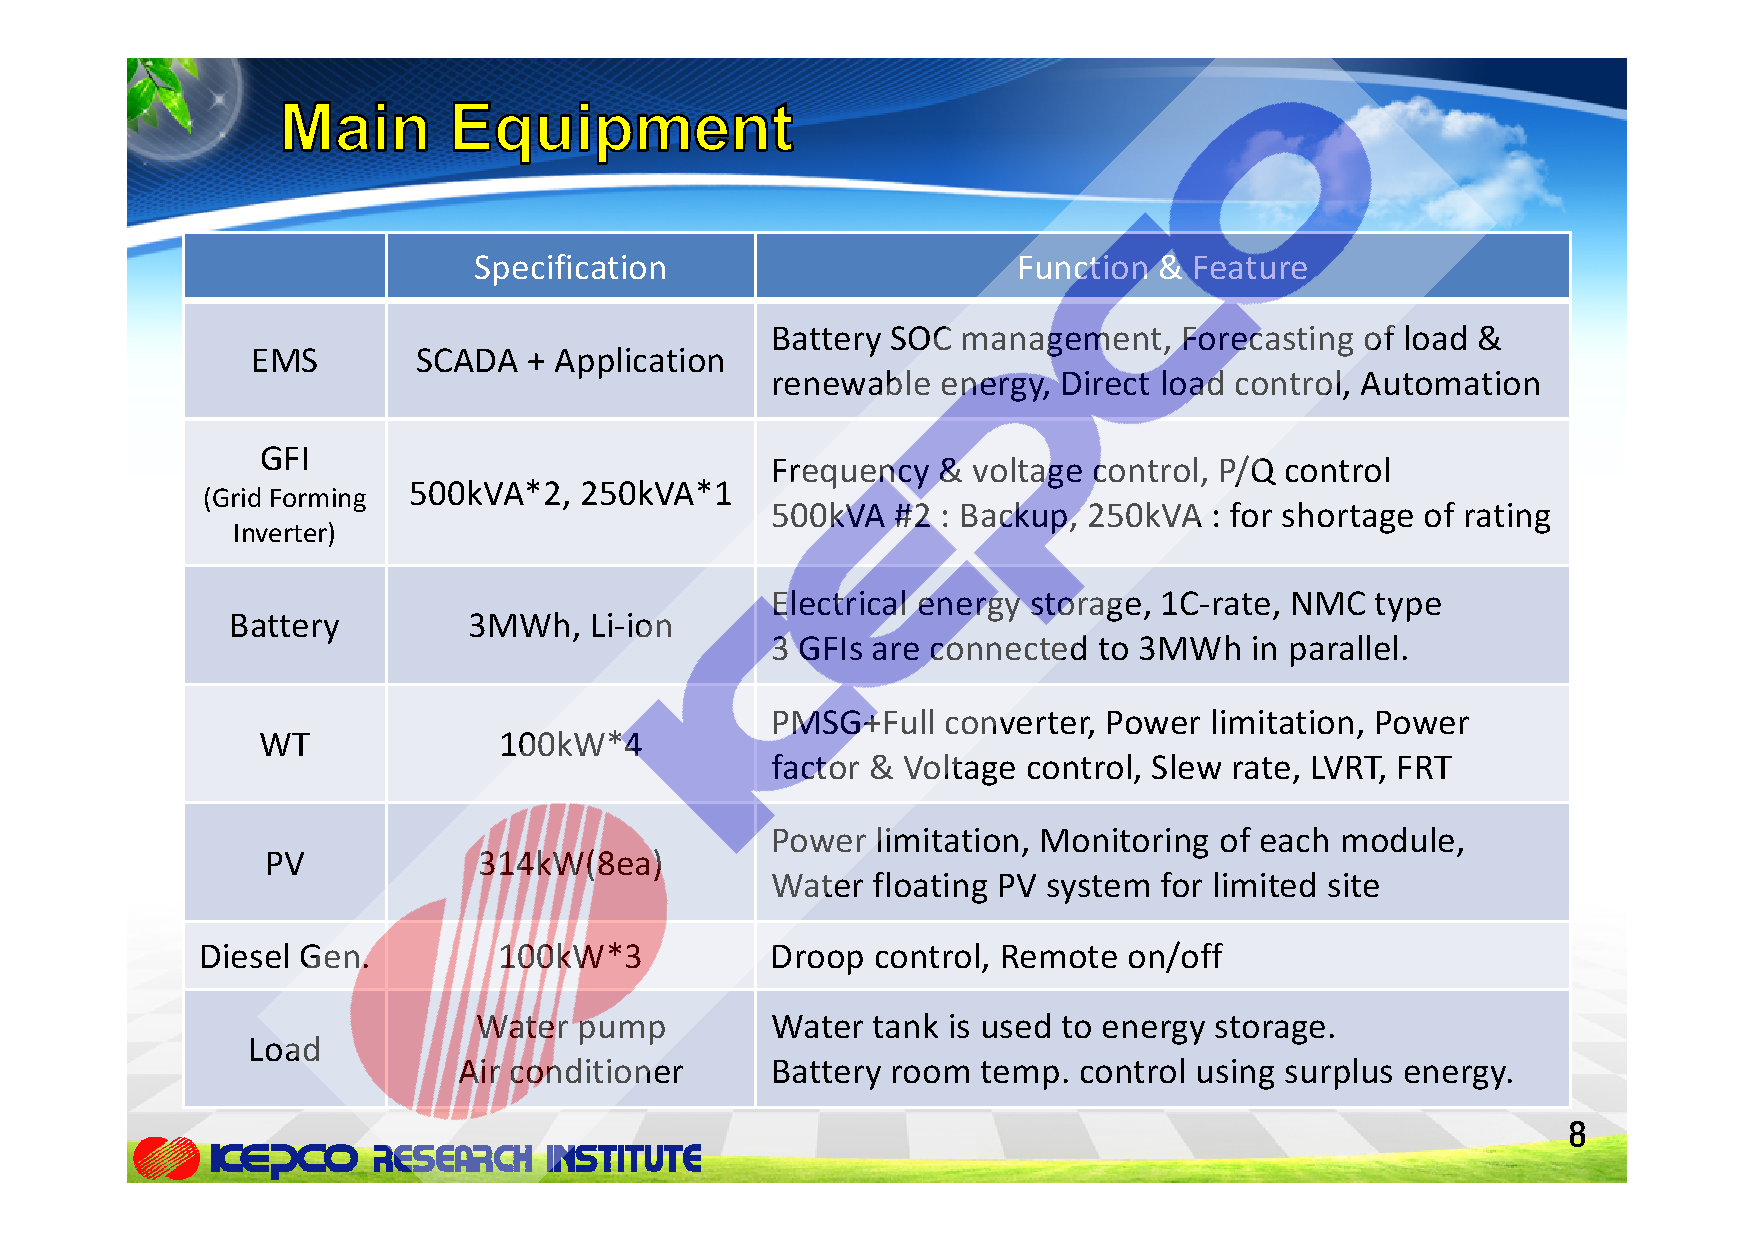
\includegraphics[width=\hsize]{KEPCO-kit.pdf}
\end{frame}


% nowcasting
\section{Solar Nowcasting}

\begin{frame}\frametitle{Solar nowcasting}
  \begin{itemize}
  \item Predicting solar output for the next 2-30 minutes.
    \pause
  \item Long history of research and development,
    including projects in Darwin 15 years ago.
    Vast number of projects on the big grid.
    Australia has around 4 studies funded in the area.
    \pause
  \item Researchers: UCSD, NUS, CSIRO, ANU,...
    \pause
  \item   And a few commercial suppliers:
    Fulcrum 3D, Pixel Sciences, Reuniwatt,...
  \end{itemize}
\end{frame}

\begin{frame}\frametitle{PV for 1 week}
There are good days and bad days:

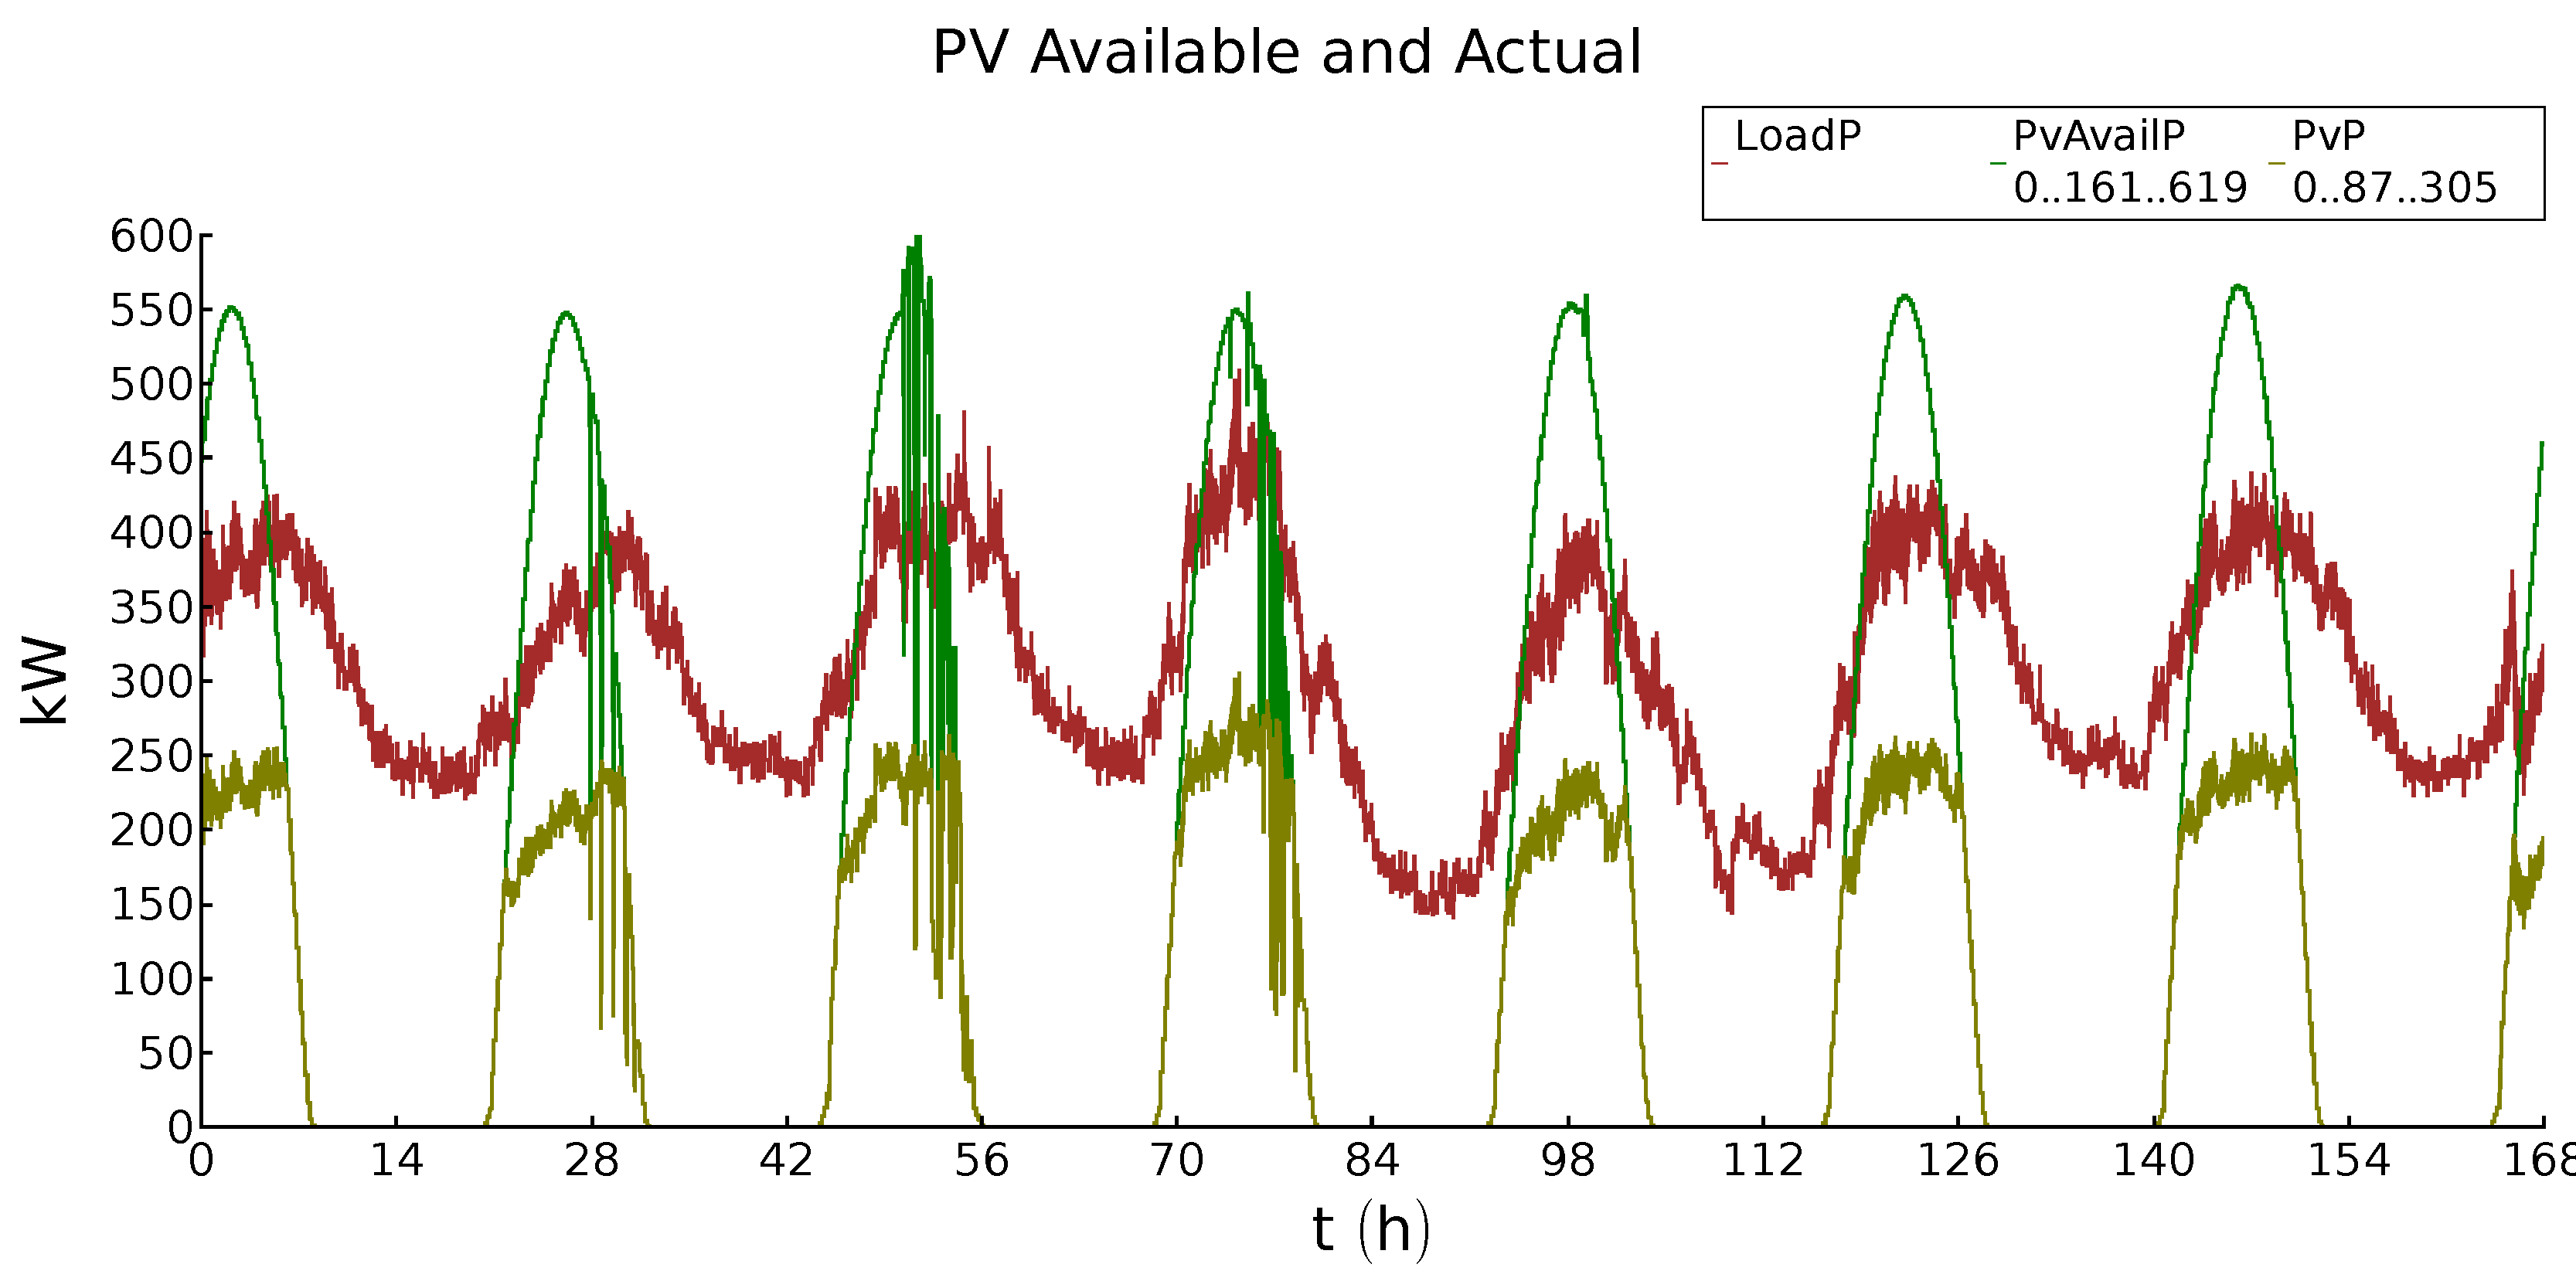
\includegraphics[width=9cm]{figPv1.pdf}
\end{frame}

\begin{frame}\frametitle{PV variation for 1 week}
And a good days variation is less than spinning reserve:

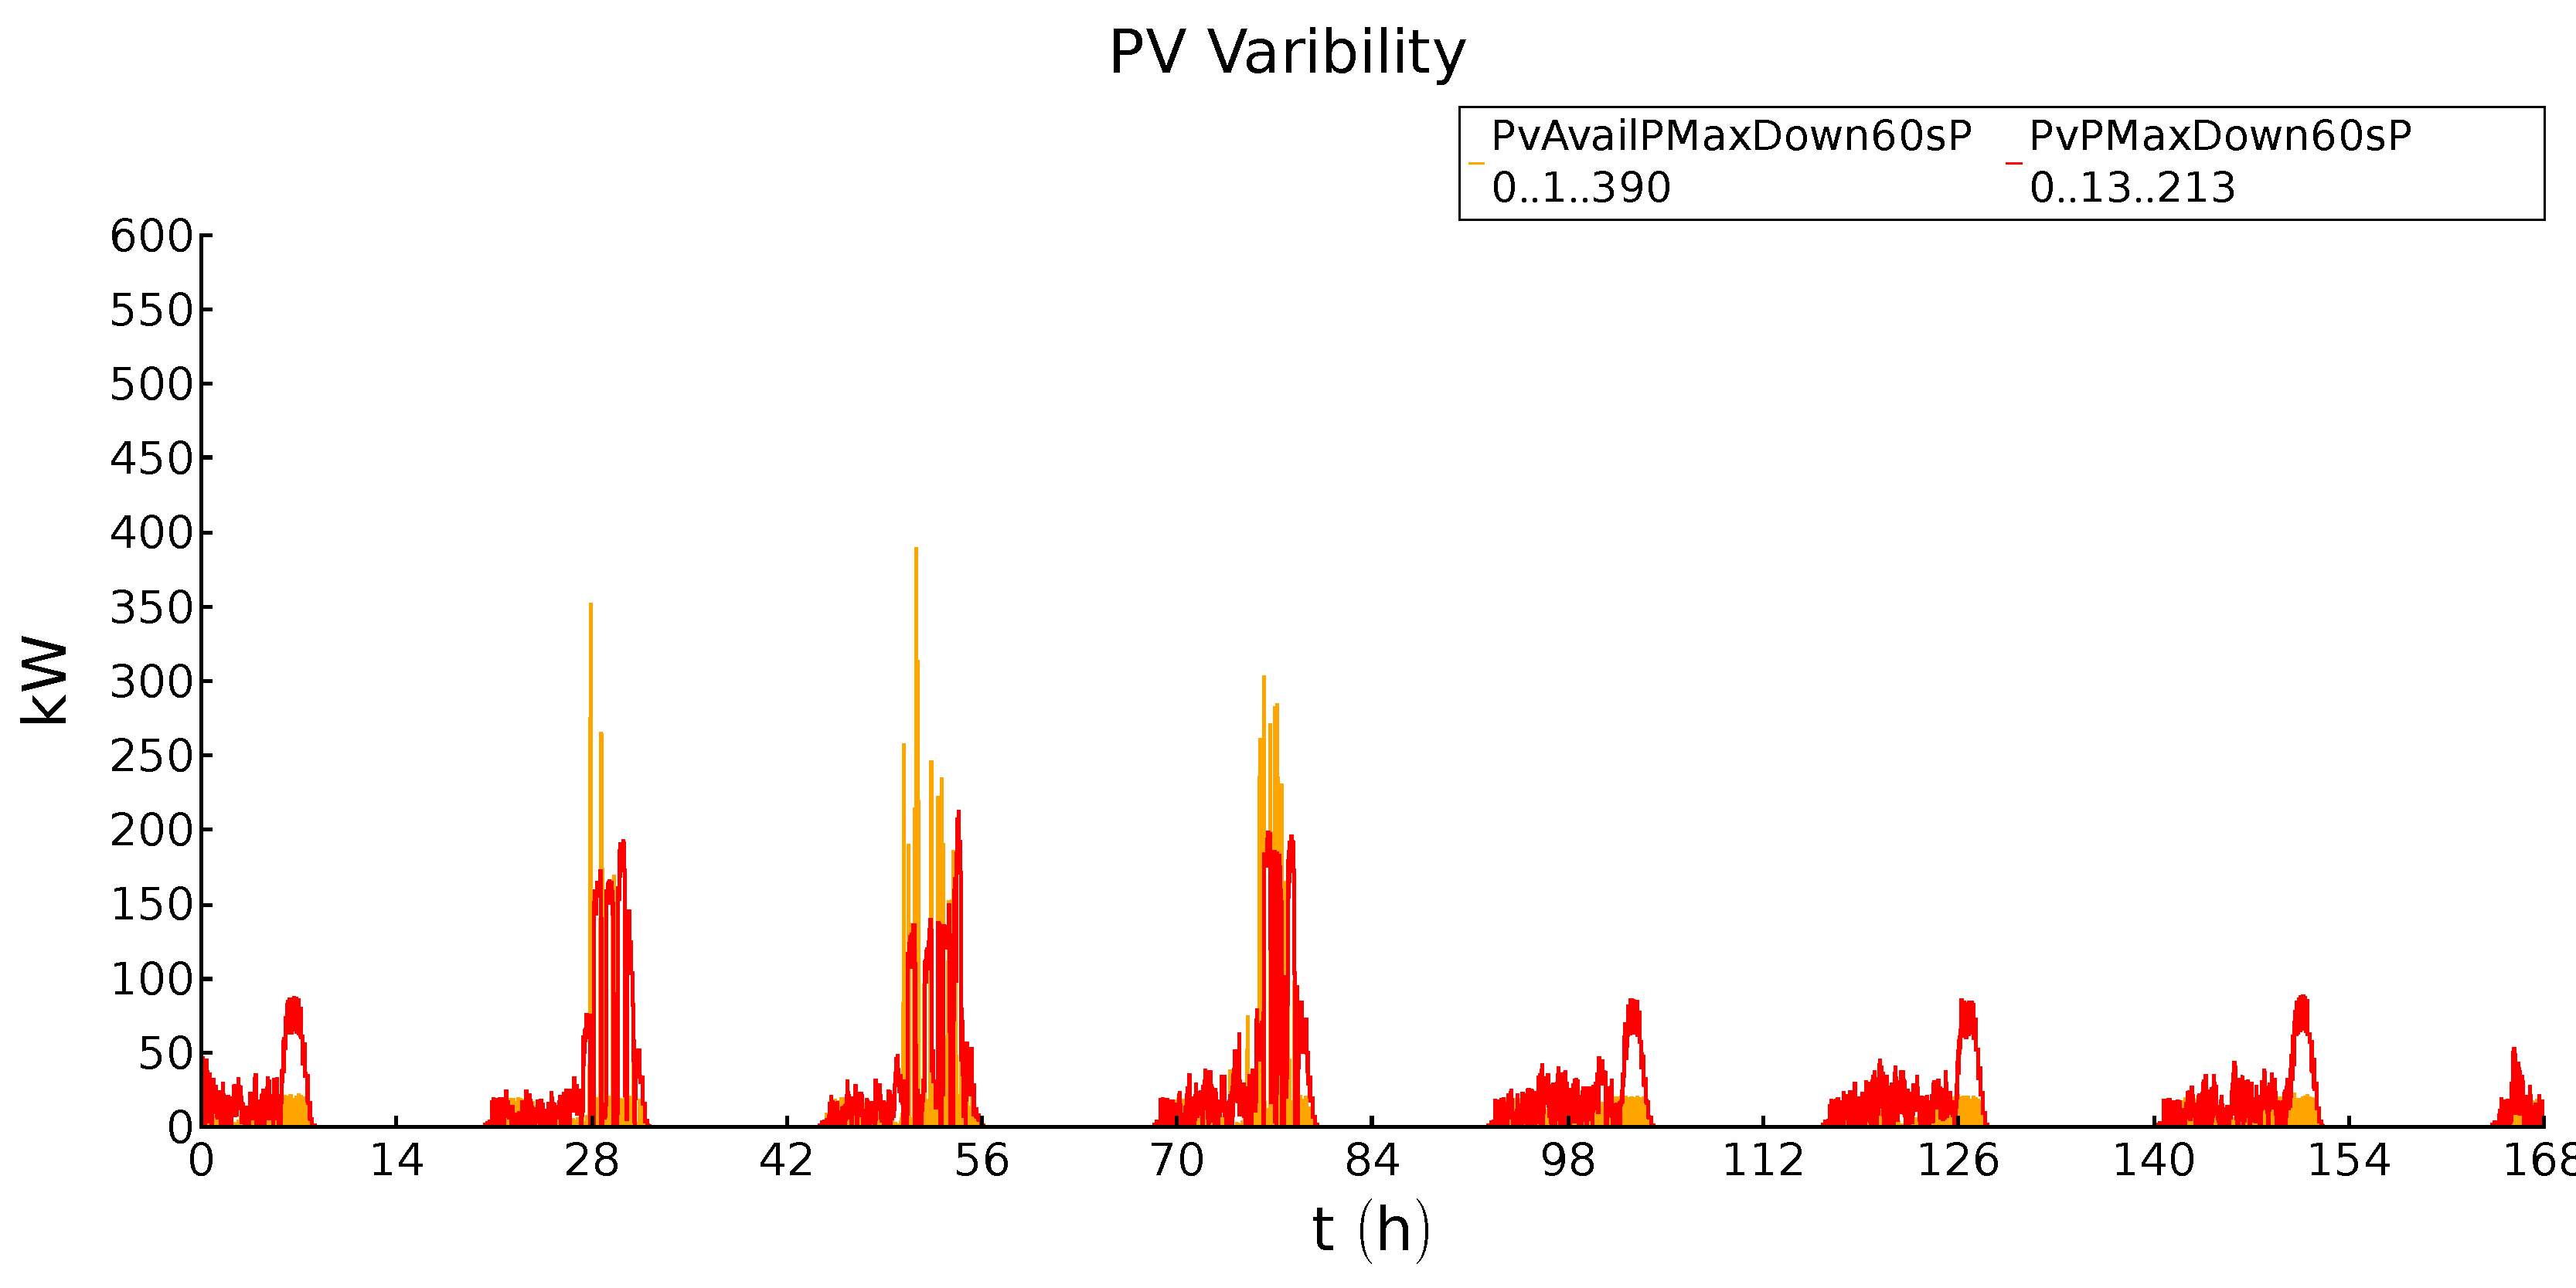
\includegraphics[width=9cm]{figPv2.pdf}  
\end{frame}


\begin{frame}\frametitle{So what}
  \begin{itemize}
  \item Assume 3 x 320kW generators with a minimum loading
    of 50\% (160kW). 
  \item Typical loading in 240..500kW range
    and 350kW PV installed. 
  \item Assuming 100\% PV coverage (no storage).
    \pause
  \item So without/with a sky camera doing now casting we get:
  \begin{center}
    \begin{tabular}[c]{|l|l|l|l|l|l|l|} 
      \hline
      SkyCam & Load kW & Gens & Gen kW & Pv kW & L/h & L/kWh \\
      \hline
      No      & 350     & 2     & 320   & 30    & 90 & 0.26 \\
      Yes     & 350     & 1     & 160   & 190   & 45 & 0.13 \\
      \hline
      No      & 500     & 2     & 320   & 180   & 90 & 0.18 \\
      Yes     & 500     & 1     & 160   & 340   & 45 & 0.09 \\
      \hline
    \end{tabular}
  \end{center}
  \pause
  \item So 200 d/y for 6h/d saving 45L/h at 1\$/L is \pause
    54k\$/y \pause by 50\% for luck = reasonable amount.
  \end{itemize}

\end{frame}

\begin{frame}\frametitle{SkyCam Procurement}
Yet another model for procurement (for us at least:\footnote{Thanks to Tim Powe}).
  \begin{itemize}
  \item 3 x Trial Systems at a target price of 15k\$.for 3..6 months.
    \pause
  \item Everyone must provide a price for a:
    \begin{itemize}
    \item Trial system for 12 months.
    \item Rollout out of from 1..10 units over the next 2 years.
    \end{itemize}
  \item The plan is for the trial results and methods to be made
    public (anyone interested).
  \end{itemize}
\vfill
  \begin{quote}
    ``Amateur project managers talk about strategy, \\
    experts talk about procurement (or logistics)'' -- Unknown
  \end{quote}
\end{frame}


% Fulcrum
\begin{frame}\frametitle{Fulcrum 3D}
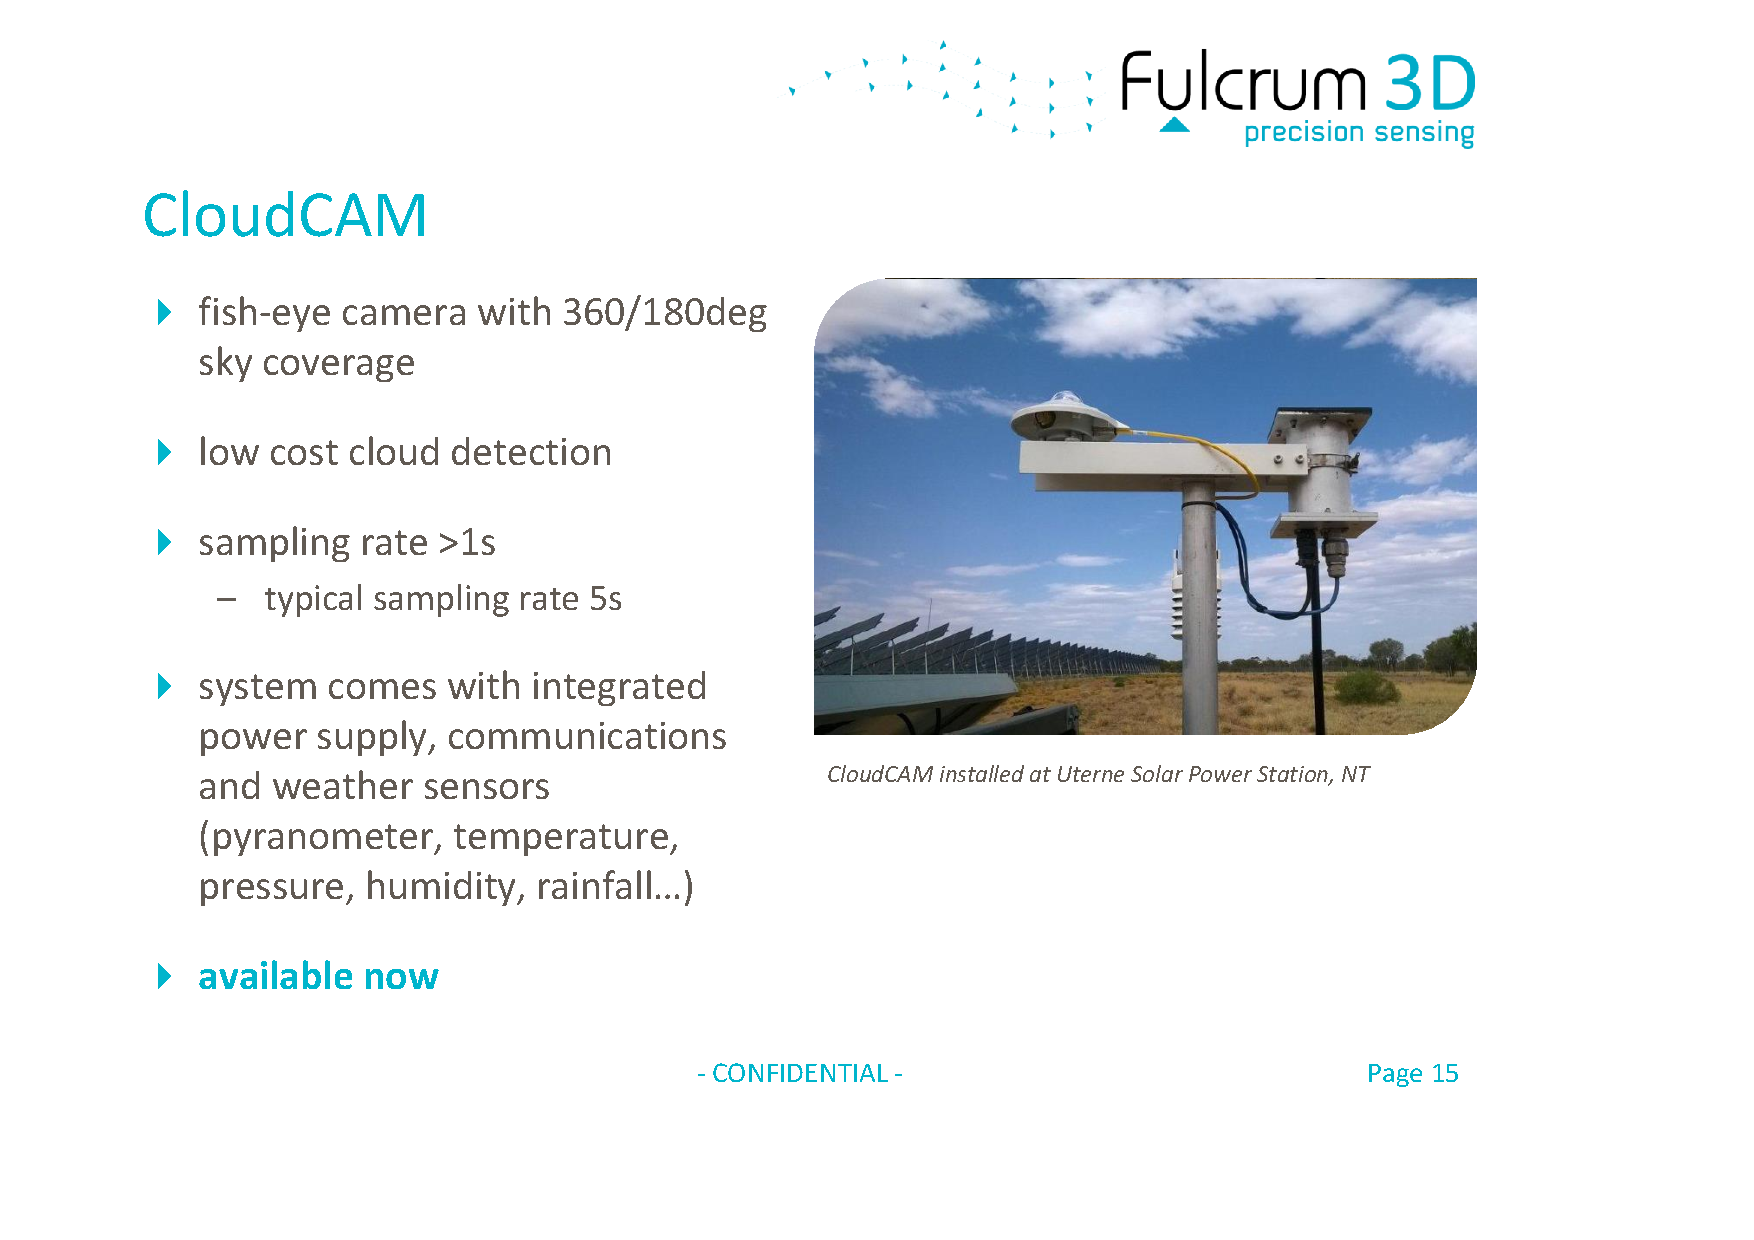
\includegraphics[width=\hsize]{Fulcrum-s1.pdf}
\end{frame}
\begin{frame}\frametitle{Fulcrum 3D}
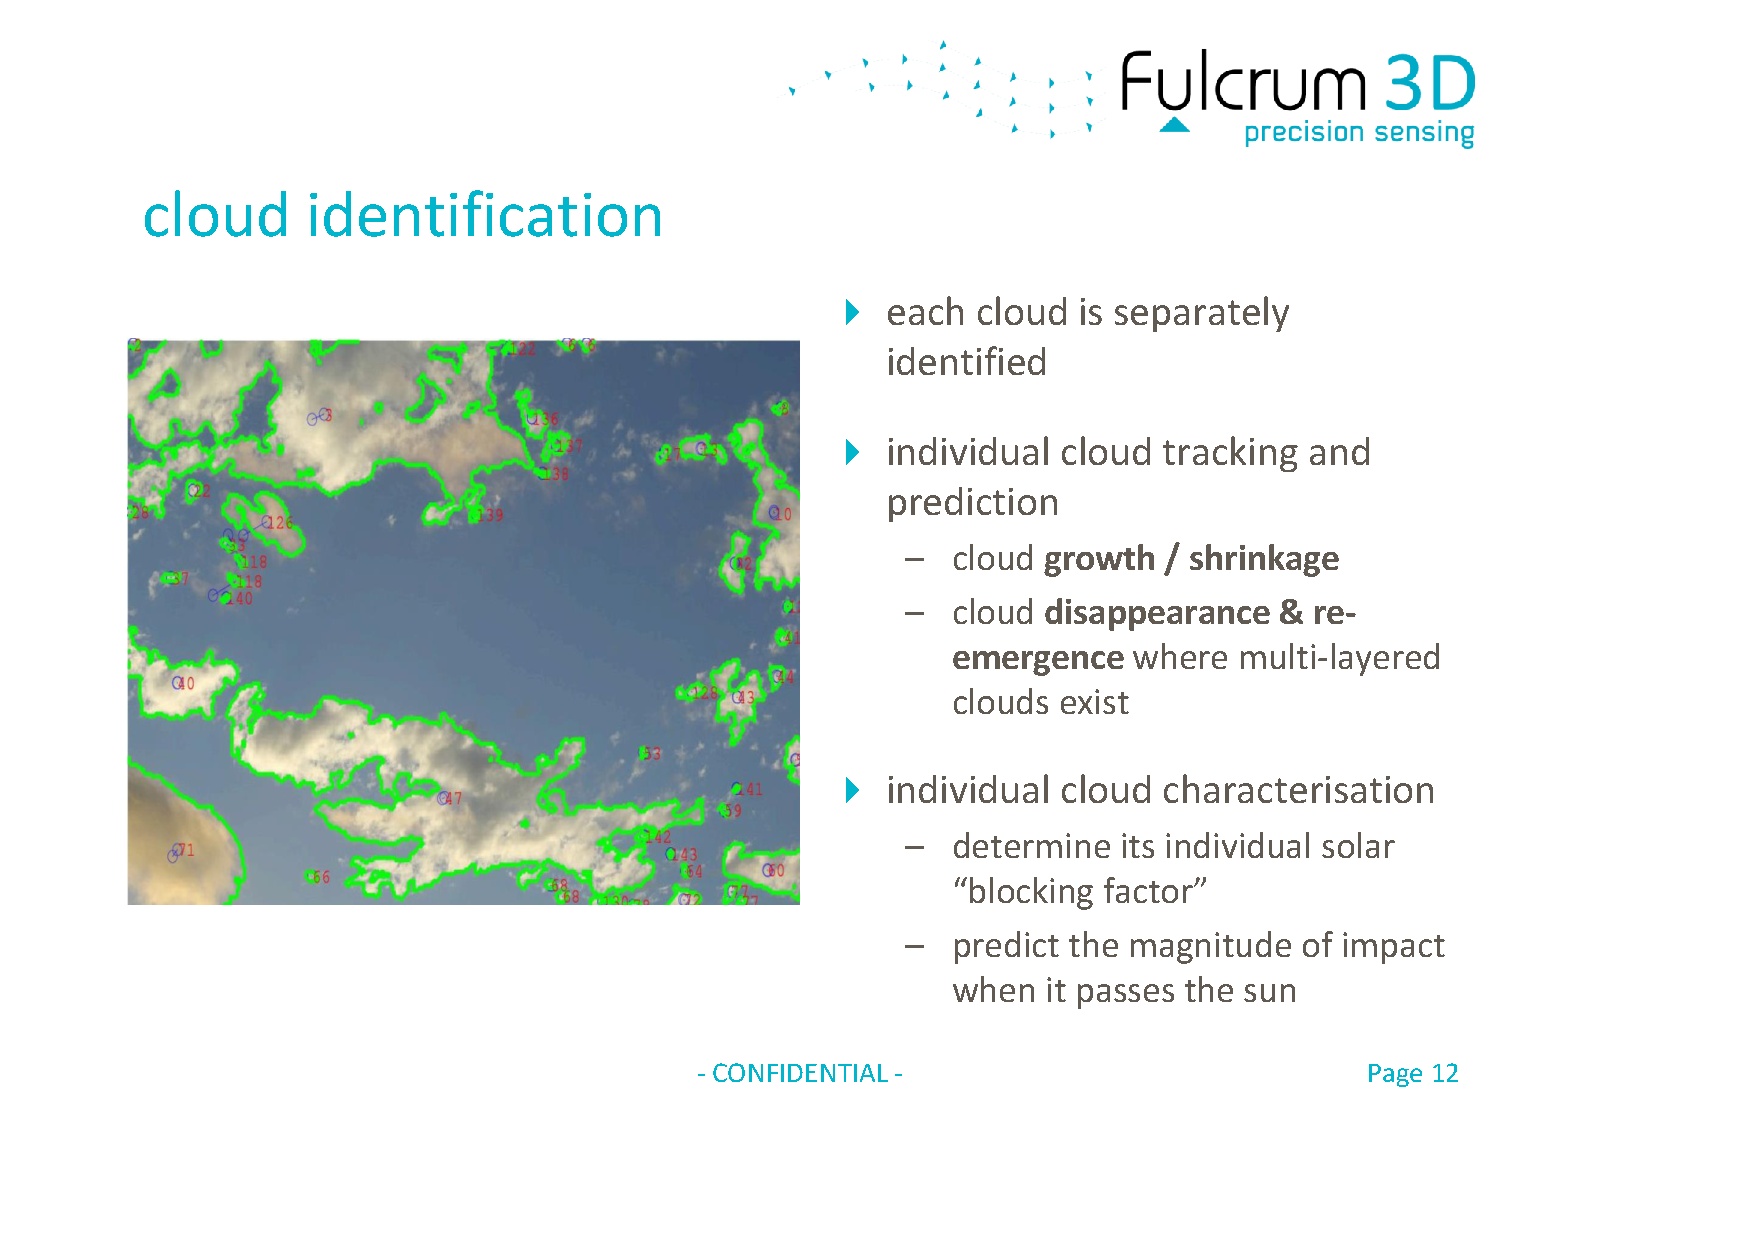
\includegraphics[width=\hsize]{Fulcrum-s2.pdf}
\end{frame}
\begin{frame}\frametitle{Fulcrum 3D}
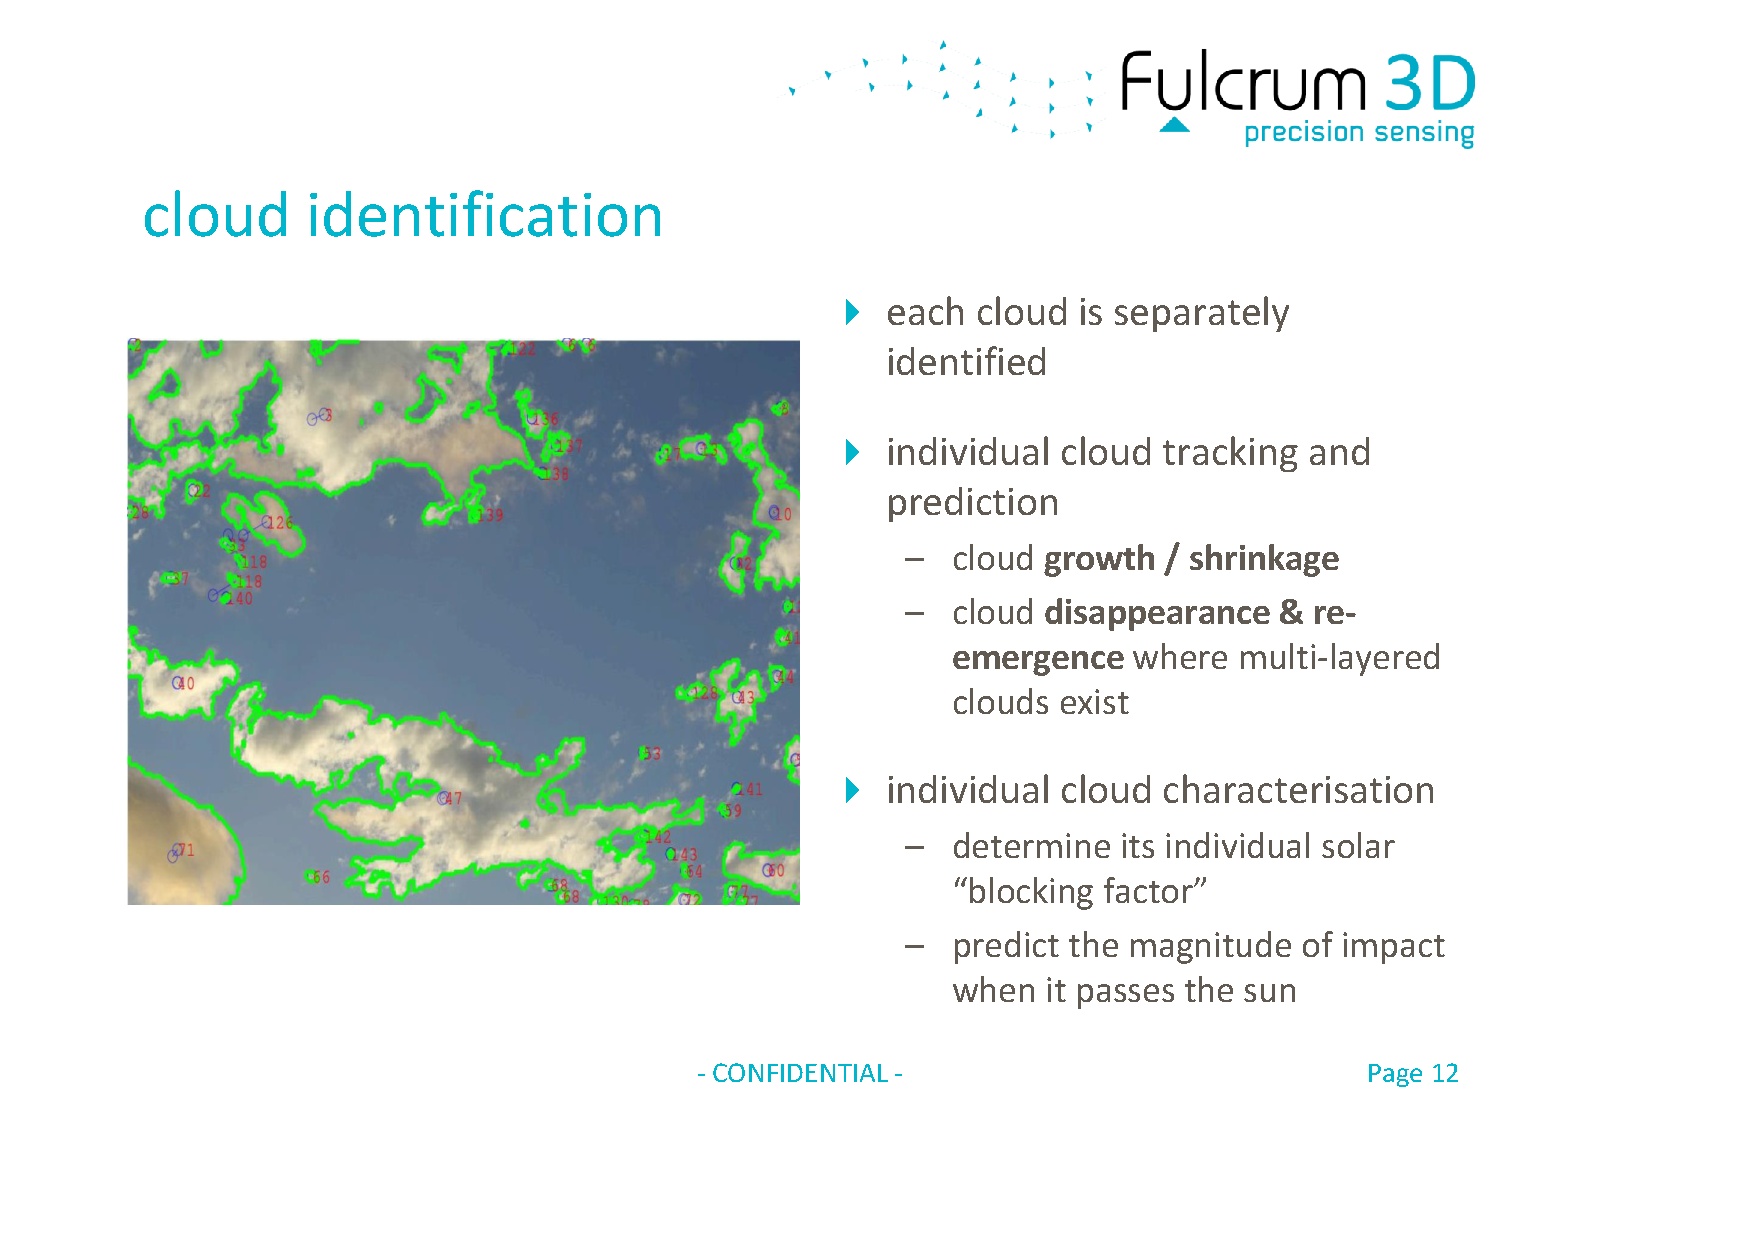
\includegraphics[width=\hsize]{Fulcrum-s3.pdf}
\end{frame}

% Pixel Science
\begin{frame}\frametitle{Pixel Science}
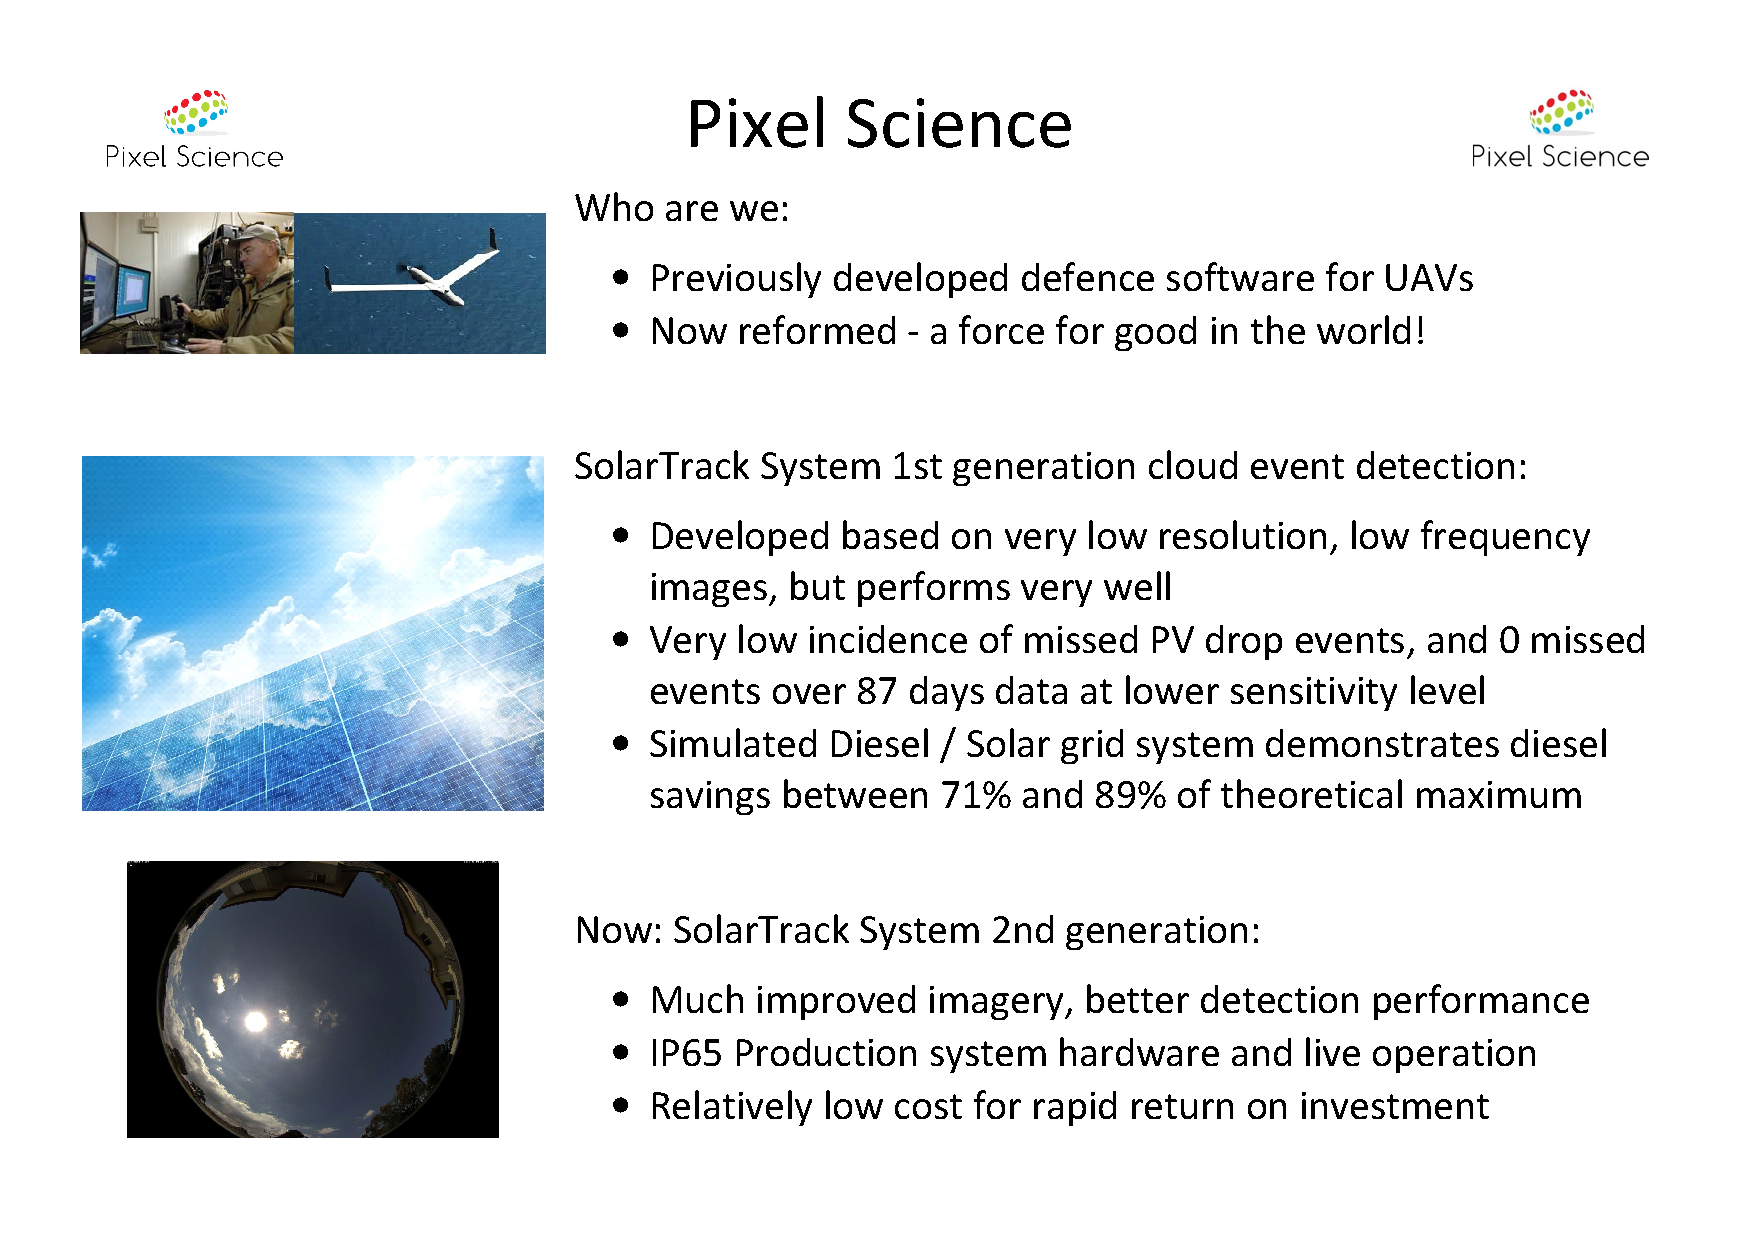
\includegraphics[width=\hsize]{PixelScience.pdf}
\end{frame}

% Reuniwatt
\begin{frame}\frametitle{Reuniwatt}
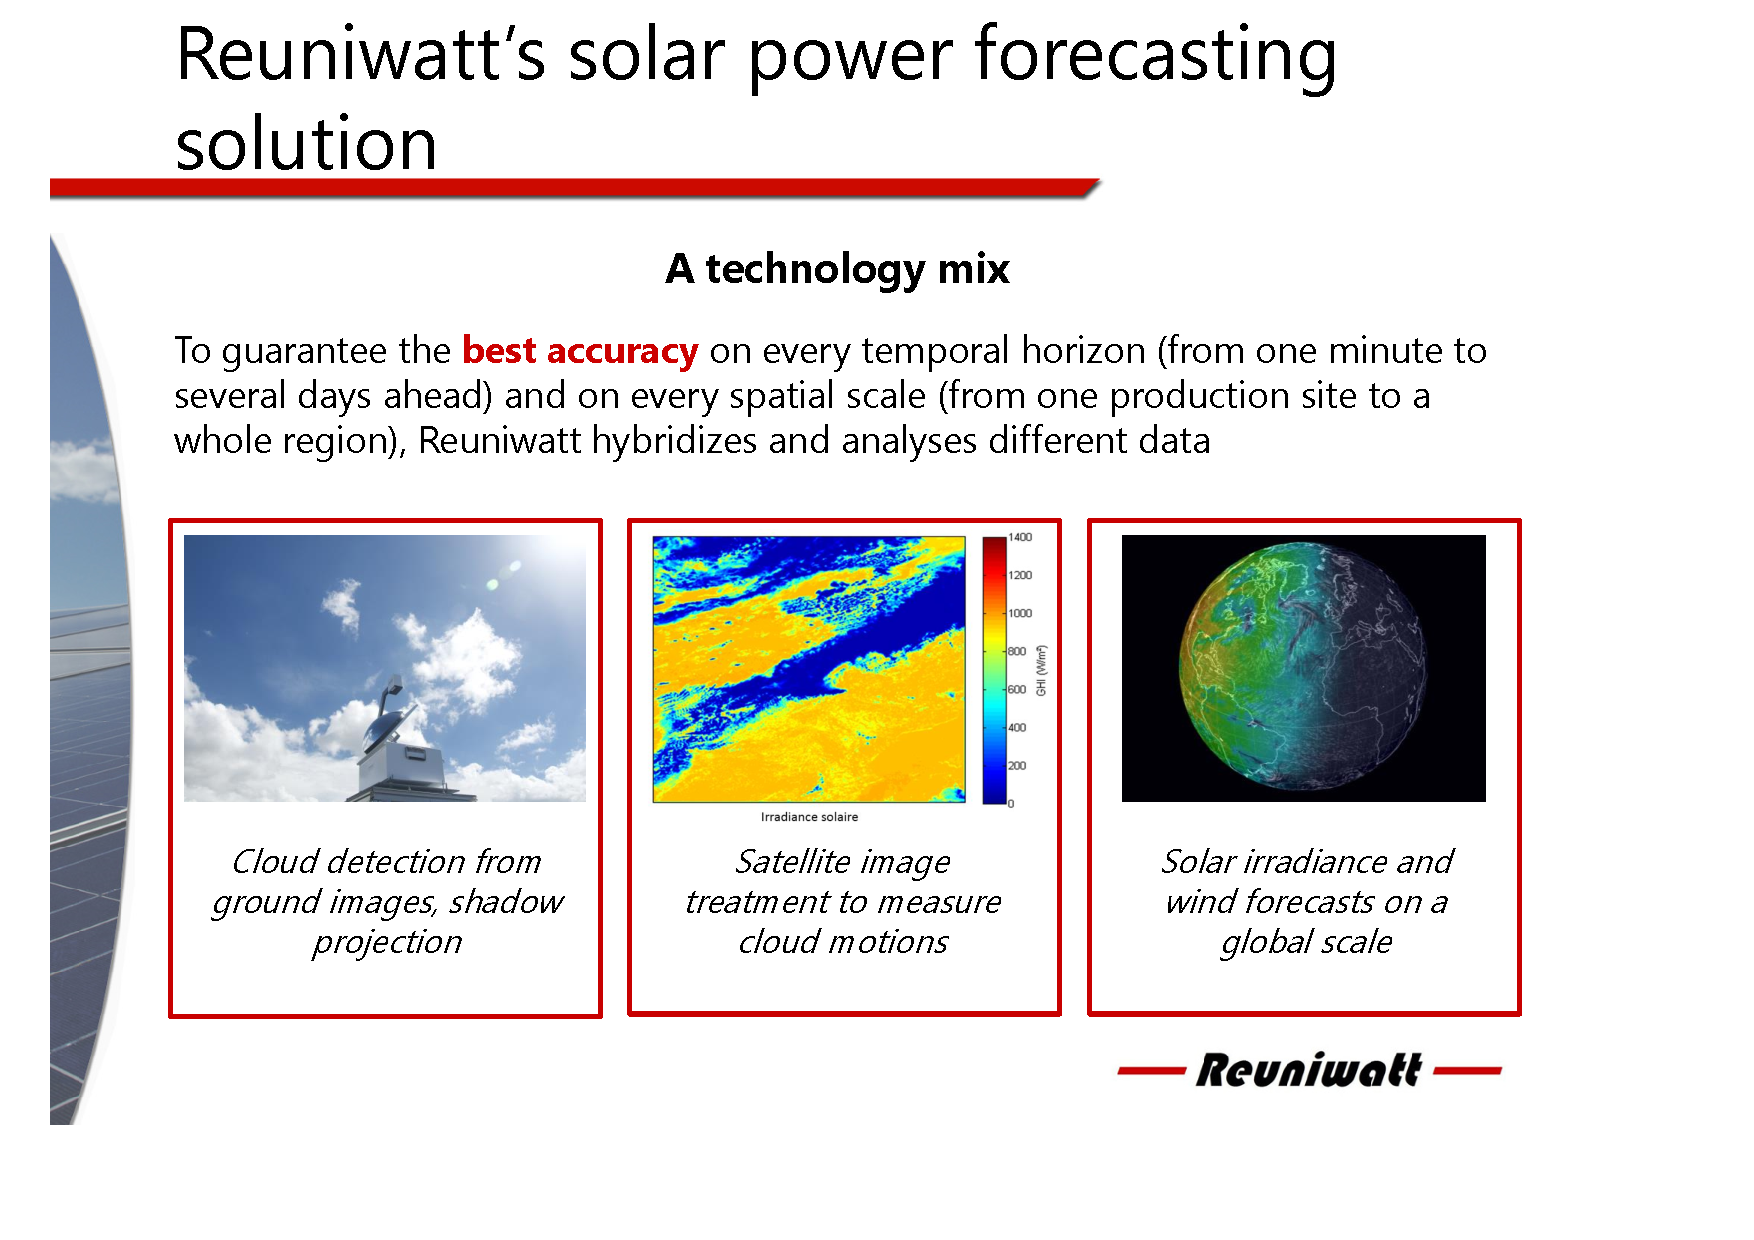
\includegraphics[width=\hsize]{Reuniwatt_Nowcasting1.pdf}
\end{frame}

\begin{frame}\frametitle{Reuniwatt}
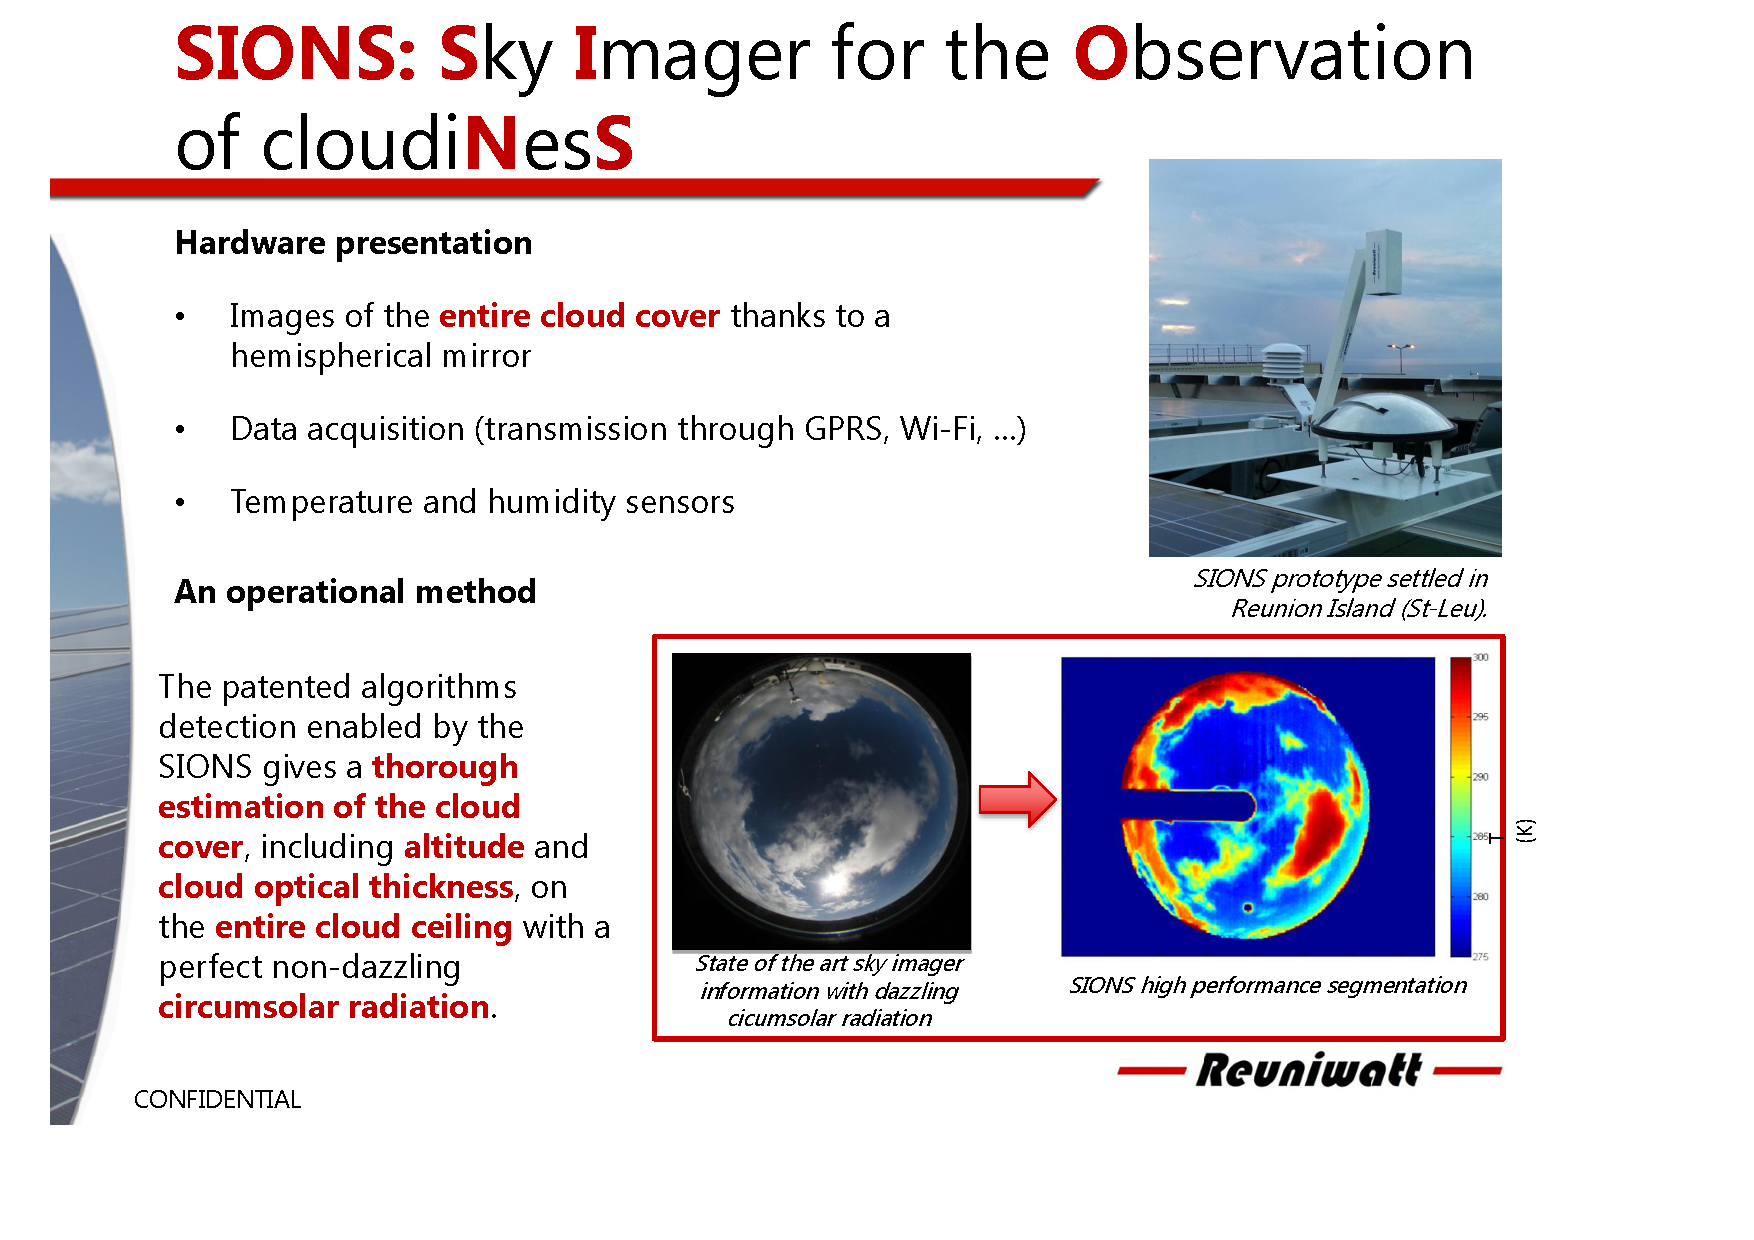
\includegraphics[width=\hsize]{Reuniwatt_Nowcasting2.pdf}
\end{frame}

\section{Lessons Learnt}
\begin{frame}\frametitle{Lessons Learnt}

\begin{enumerate}
\item Solar Forecasting \emph{may} be an answer for part of the
  problem. Results to be available next year.
\pause
\item There are a lot of interesting experiences from the 
  southern part of the world in hybrid systems.
\pause
\item Development evaluation, procurement, and testing 
  are all required for successful systems.
\pause  
\item Be very careful when you say X is the biggest for any X.
\end{enumerate}
\pause
\vfill
\begin{quote}
``Economics are the method; 

\pause
the object is to change the heart and soul'' -- Thatcher
\end{quote}
\end{frame}
\end{document}

